
%\subsection{Architek}
\begin{frame}
  \frametitle{P2P Chord}
  \framesubtitle{Idee}
  \begin{itemize}
    \item Chord-Architektur ist ein verteiltes Hashtabelle-System
    \item Basiert auf strukturierten Overlay-Netzwerk
    \item Bekannt seit 2001
    \item Grundlage für die Entwicklung von Blockchain-Technologien 
    \item Grundlage dezentralisierten autonomen Organisationen (DAOs) 
  \end{itemize}
\end{frame}

\begin{frame}
  \frametitle{P2P Chord}
  \framesubtitle{Struktur und Funktionsweise}
  \begin{itemize}
    \item Identifier Space: Default Ring
    \item Key-Node Mapping
    \item Finger Tables
    \item Lookup-Operationen
    \item Dynamik und Fehlertoleranz
  \end{itemize}
\end{frame}

\begin{frame}
  \frametitle{P2P Chord}
  \framesubtitle{Einsatzmöglichkeiten}
  \begin{itemize}
    \item Dateifreigabe
    \item Distributed Domain Name System (DDNS)
    \item Content Distribution Networks (CDN)
    \item Distributed Databases
    \item etc
  \end{itemize}
\end{frame}

\begin{frame}
  \frametitle{P2P Chord}
  \framesubtitle{Beispiel}
  \begin{figure}[!ht]
    \centering
    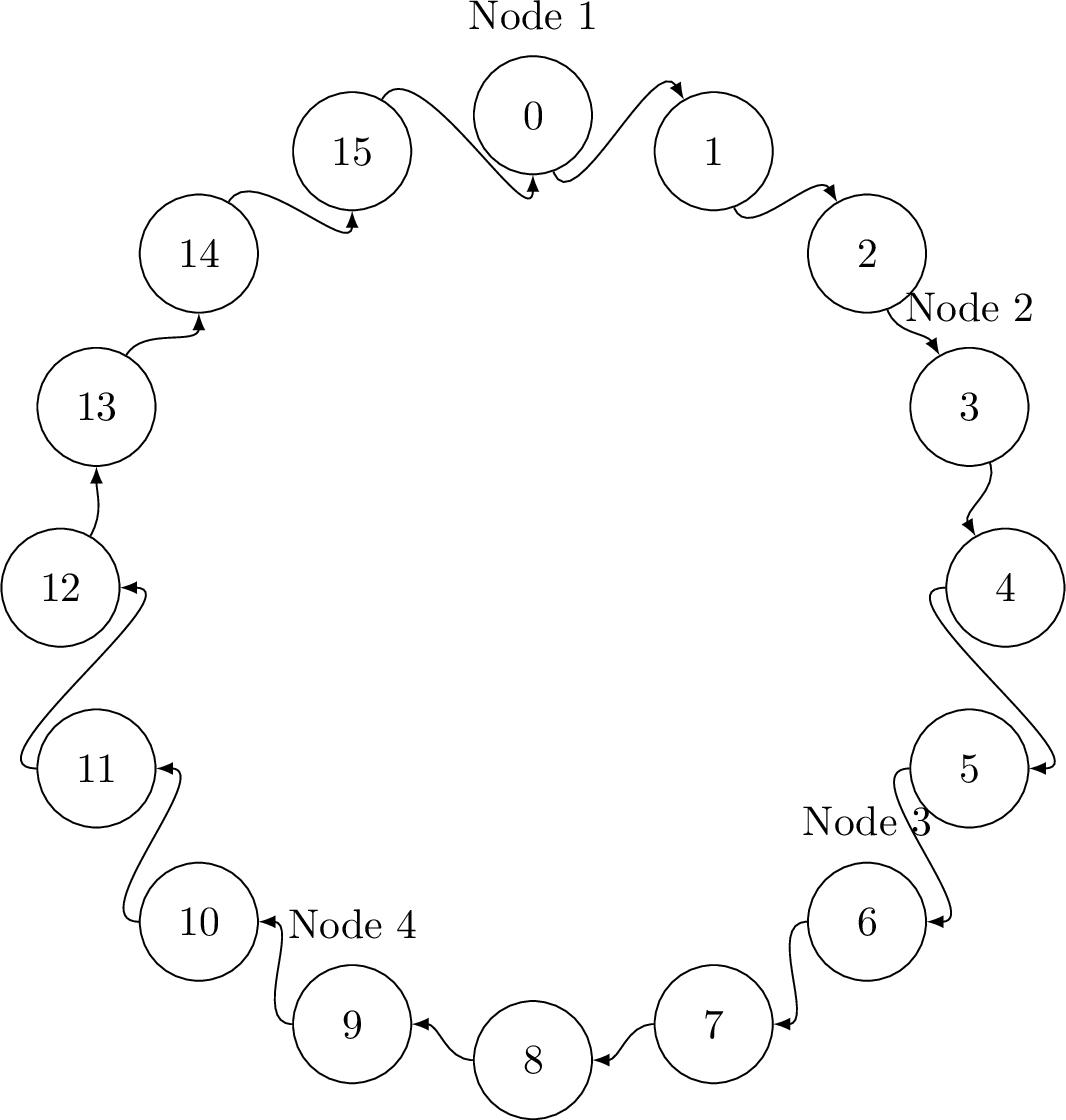
\includegraphics[width=0.45\textwidth]{fig/tex-grapics/chord.pdf.png}
    \caption{Chord Setup}
    \label{fig:chord}
  \end{figure}
\end{frame}

\begin{frame}
  \frametitle{P2P Chord}
  \framesubtitle{Fingertable}
  \begin{itemize}
    \item $log(n)$ Einträge
    \item $(n + 2^{(i-1)}) \mod 2^m$
    \item Lässt schnelle Suche zu (im Vergleich zur linearen)
  \end{itemize}
\end{frame}

\begin{frame}
  \frametitle{P2P Chord}
  \framesubtitle{Cassandra}
  \begin{itemize}
    \item NoSQL-Datenbanksystem
    \item Partitionierungsstrategie
    \begin{itemize}
      \item Range-based Sharding
      \item Hash-based Sharding
    \end{itemize}
    \item Replikationsstrategie
    \item Datenmodell
    \item Gossip-Protokoll (statt Fingertable für Routing-Aufbau)
    \item Hinted Handoff
    \item Repair und Anti-Entropy
  \end{itemize}
\end{frame}